\section{Methods}
%	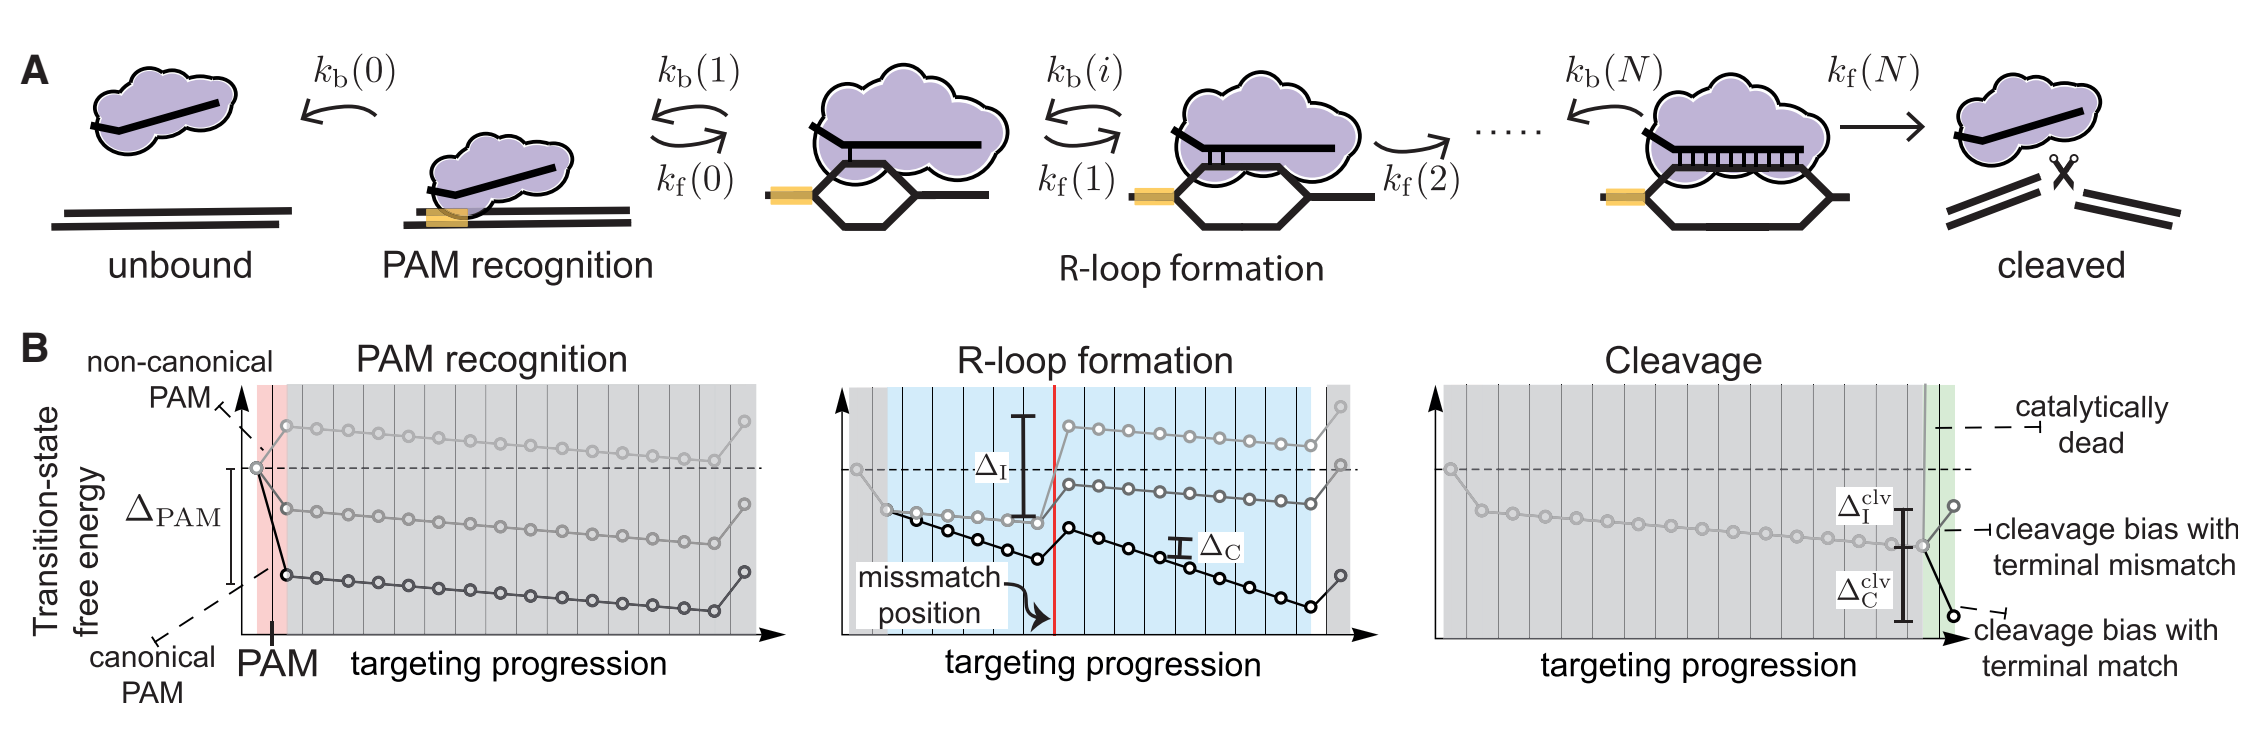
\includegraphics[width=5in]{1.png}
\subsection{Kinetic module}
Figure \ref{fig:2} shows that the whole binding-cleavage process begins with the binding between PAM and protein. Therefore, it corresponds to rule 1 mentioned before. And as the reaction proceeds, every step of it is reversible, and its irreversibility mainly depends on the binding energy of two DNA bases.
\begin{figure}
\centering
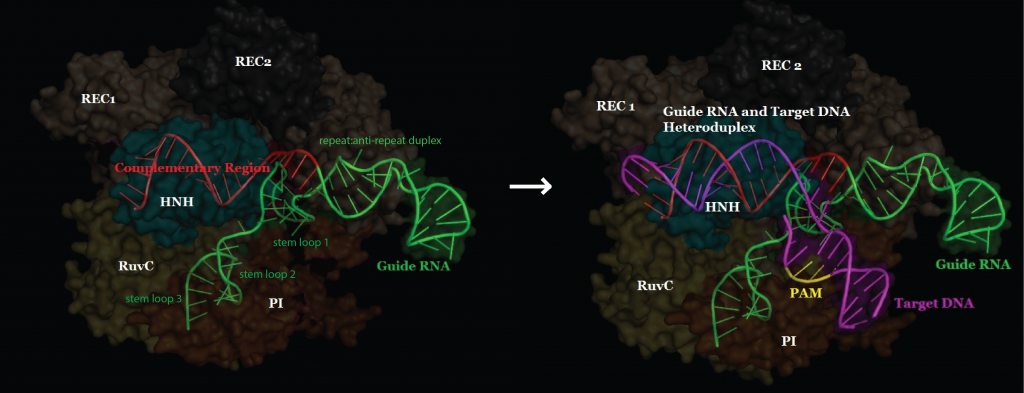
\includegraphics[width=0.7\linewidth]{2}
\caption{}
\label{fig:2}
\end{figure}

\begin{figure}
\centering
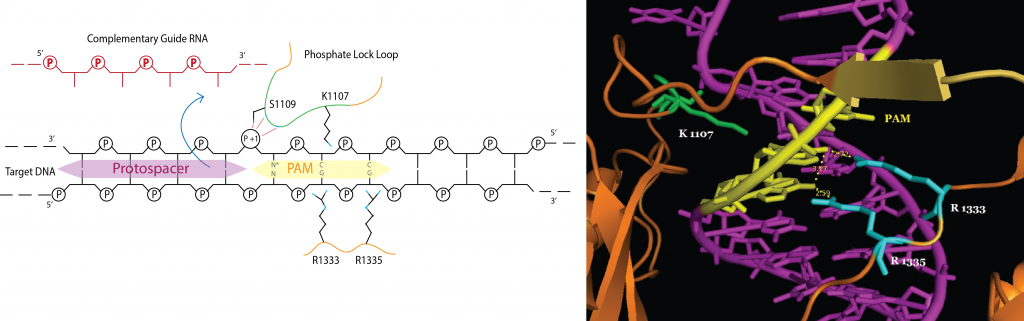
\includegraphics[width=0.7\linewidth]{3}
\caption{}
\label{fig:3}
\end{figure}

\begin{figure}
\centering
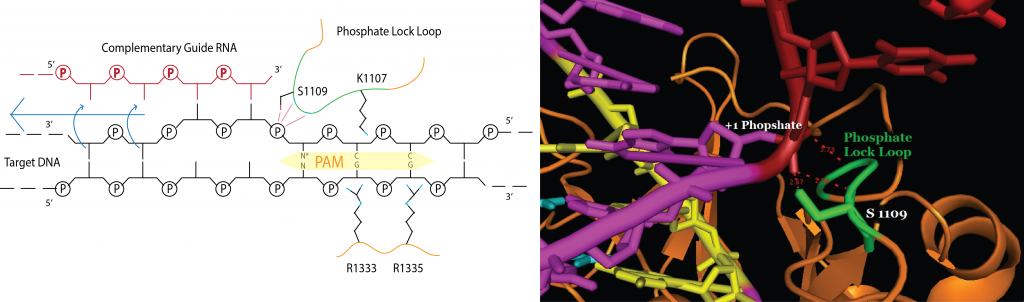
\includegraphics[width=0.7\linewidth]{4}
\caption{}
\label{fig:4}
\end{figure}

\begin{figure}
\centering
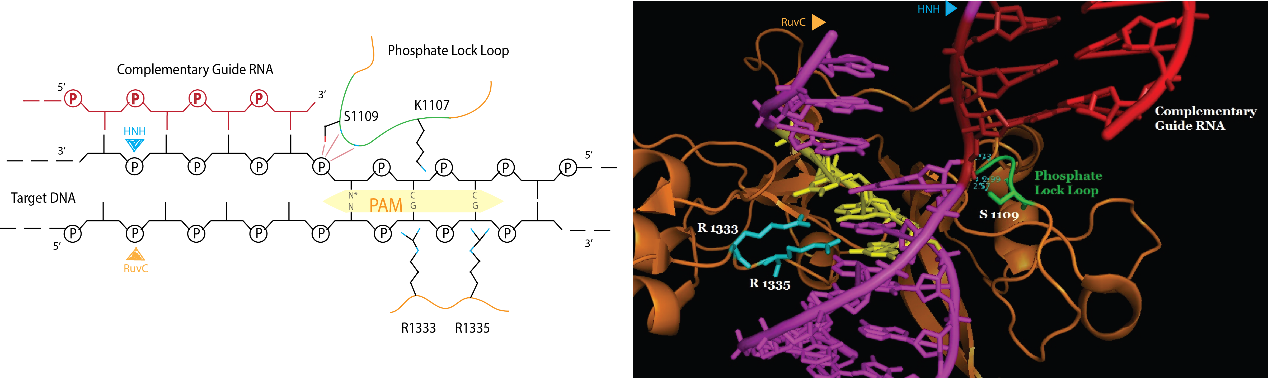
\includegraphics[width=0.7\linewidth]{5}
\caption{}
\label{fig:5}
\end{figure}
	
The boundary probability $P_{clv;N}$ , representing the probability of matching at the Nth position (the last position of sgRNA) of nucleotide base, is given by:
\begin{equation}
P_{m,N}=\frac{k_f(N)}{k_f(N)+k_b(N)}=\frac{1}{1+\gamma_N} \quad
\end{equation}
where $k$ is the reaction rate constant; $f$ represents the forward reaction; $b$ represents the backward reaction. And 
\begin{equation}
 \gamma_N=\frac{k_b(N)}{k_f(N)}
\end{equation}
So for a complete match: 
\begin{equation}
P_{m} \equiv P_{m,0} = \frac{1}{1+\sum_{n=1}^N\coprod_{i=1}^n \gamma_i}
\end{equation}
Consider the rate constant $k_f(i)$ and $k_b(i)$:
\begin{equation}
k_f(i)=k_0exp(-(T_{i,i+1}-F_i)),k_b(i)=k_0exp(-(T_{i,i-1}-F_i))
\end{equation}
where $F_i$ means free energy of each metastable state, $T_{i,i+1}$ means the highest free energy point on the reaction path from position i to position i + 1. Therefore, $T_{i,i+1}-F_i$ is the activation energy of forward reaction and $T_{i,i-1}-F_i$ is activation energy of the backward reaction.
\begin{equation}
\Rightarrow \gamma_i=exp(-\Delta_i), \Delta_i=T_{i,i+1}-T_{i,i-1}
\end{equation}
\begin{equation}
\begin{aligned}
\Rightarrow P_{m} = \frac{1}{1+\sum_{n=1}^N\coprod_{i=1}^n \gamma_i}=\frac{1}{1+\sum_{n=1}^N\coprod_{i=1}^n exp(-\Delta_i)}\\=\frac{1}{1+\sum_{n=1}^N exp(-\sum_{i=1}^n\Delta_i)}
\end{aligned}
\end{equation}
We define $$\Delta T_n=\sum_{i=1}^n\Delta_i$$
so
\begin{equation} 
P_{m} =\frac{1}{1+\sum_{n=1}^N exp(-\Delta T_n)}
\end{equation}
	
From the above, it is clear that the matching probability depends only on the state transition energy, not on the free energy of the metastable states. If we assume there is one dominant minimal bias, say for $n = n^*$, then this equation can be approximated as:
\begin{equation}
 P_{m} \approx \frac{1}{1+exp(-\Delta T_{n^*})}
\end{equation}

As figure shows, we analyze each process energy change:\newline
$\left\{
\begin{tabular}{l}
for the PAM state (i = 0) we have $\Delta_0=\Delta PAM$\\
for a partial R-loop we have $\Delta_i = \Delta_C$ and $\Delta_i = -\Delta_I$ if mismatched\\
\end{tabular}
\right.$

\begin{equation}
\Delta {T_n} = {\Delta _{PAM}} + {n_C}(n){\Delta _C} - (n - {n_C}){\Delta _I} - {\delta _{n,N}}{\Delta _{clv}};\:n = 0...N
\end{equation}
where $\delta_{n,N}$ represents the Kronecker delta:
$\delta_{n,N}$=$\left\{\begin{array}{l}1, n=N;\\
0, n\neq N.
\end{array}
\right.$\\
For PAM independent systems (such as Cas13), we instead use:
\begin{equation}
\Delta {T_n} = {n_C}(n){\Delta _C} - (n - {n_C}){\Delta _I} - {\delta _{n,N}}{\Delta _{clv}};\:n = 0...N
\end{equation}

To sum up, the cleavage possibility mainly relies on the free energy change, and PAM appears as a significant energy decline.
\begin{figure}[h]
	\centering
	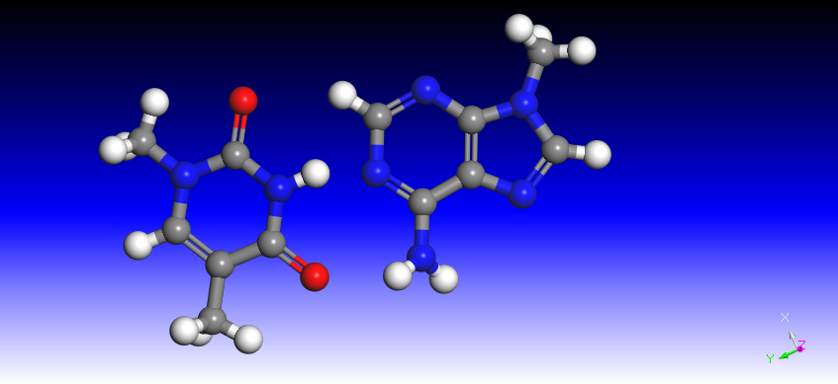
\includegraphics[width=0.7\linewidth]{AT}
	\caption{AT}
	\label{fig:6}
\end{figure}
\begin{figure}[h]
	\centering
	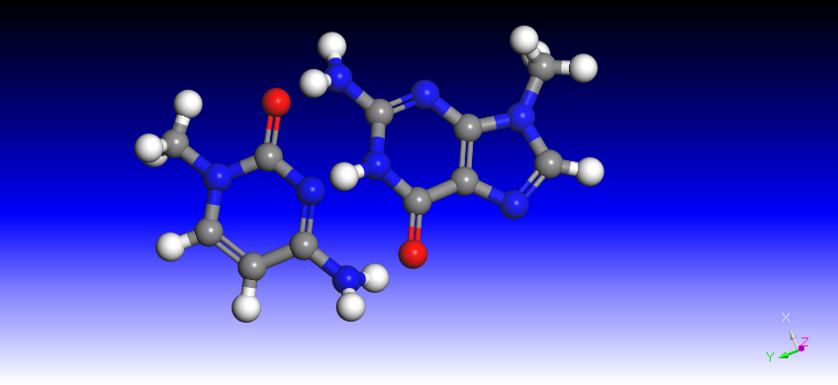
\includegraphics[width=0.7\linewidth]{CG}
	\caption{CG}
	\label{fig:7}
\end{figure}

So the kinetic module set up a form to regress the relationship between cleavage and the numbers of nucleotide matches and mismatches.
In consideration of this problem more carefully, the cleavage possibility becomes equal to analysis energy change, and we know the binding energy of A/T and C/G is different due to the different hydrogen bond between them. However, in appearing kinetic model, research tend to describe them in a rough definition as “matched base pairs”, and the energy incline in C/G is approximately 1.5 folds as A/T. Similarly, the mismatch has more difference because the size of nucleotides is various. Hence, the combination of the mismatched base pair was classified by group volume, i.e. two pyrimidines (such as C/T, “L”), pyrimidine and purine (such as C/A, “M”), two purine (such as G/T, “S”). Hence, our possibility can be calculated using the following formation.
\begin{equation}
P_{clv}=\frac{1}{1+e^{-n_1\Delta_{A/T}-n_2\Delta_{C/G}+n_3\Delta_{L}+n_4\Delta_{M}+n_5\Delta_{S}}}
\end{equation}

\subsection{Optimization module}
It is a common sense that experimental results are facts, but theoretical results are only conjectures. From kinetic module, we can get an output, which is the cleavage possibility. The parameter we choose only aims to make results have discrimination, while it’s not quantitative. And in a cleavage experiment, we only have two outcomes, successful and unsuccessful. To make our prediction possibility more approximate to experiment, we regard this as a regression problem.

Here, the method we choose is stochastic gradient descent (SGD) and cross entropy. And their principle can be concluded as follows.
\begin{equation}
\theta  = \theta  - \eta {\nabla _\theta }J({x^{(i)}},{y^{(i)}},\theta )
\end{equation}
	
\begin{equation}
loss = \sum\limits_i {{y_i}\ln {y_i}}
\end{equation}
where $\theta$ means the parameters array and J means the loss function. 

Considering the difference in gradient calculation, we use difference to substitute differential aim to accelerate operating speed.\par
\begin{equation}
\frac{{dy}}{{dx}} \approx \frac{{\Delta y}}{{\Delta x}}{\rm{ = }}\frac{{y(x + \delta x) - y(x)}}{{\delta x}}
\end{equation}

By using this simple method, our model can be more vibrant, updating using newest data and becoming more reliable.

\subsection{Pre-selector}
It’s obviously that the algorithm is too complex to applying in slide in a huge DNA array. To solve this problem, we use a pre-selector to get some candidates and use previous model to compare them so that we could get a greatest target.\par
And here this pre-selector structure is very simple.
Considering use this map to reflect the similarity between target and full DNA.

\begin{equation}
f({a_{{\rm{target}}}} - {a_{{\rm{full}}}}) = {\bf{x}} = ({x_i})
\end{equation}

\begin{equation}{x_i} = \left\{ {\begin{array}{*{20}{c}}
{1,\quad \quad matched}  \\
{0,\quad mismatched}  \\
\end{array}} \right.
\end{equation}

Here, we use PAM as an input and collect the array which contain the same beginning code as PAM.

